\chapter{Aprendizaje automático y \textit{deep learning}}
\label{Chapter3}

\chapquote{
En este capítulo se introducen de forma resumida nociones teóricas
sobre aprendizaje automático y \textit{deep learning}. En el apartado
\ref{sec:introducción-aprendizaje} se define formalmente qué es el aprendizaje automático y se resume
qué tipos de aprendizaje hay. En el apartado \ref{sec:redes-neuronales} se explica qué son
las redes neuronales artificiales y el modelo de red utilizado en este
proyecto.}


\section{Introducción}
\label{sec:introducción-aprendizaje}

Mediante el uso de algoritmos de aprendizaje automático se pueden crear modelos que, a partir de una colección de datos, sean capaces de tomar decisiones. Formalmente, \cite{mitchell1997machine} define el aprendizaje automático como
``Se dice que un programa aprende de la experiencia E respecto a un tipo de trabajo T con una medida de rendimiento R, cuando el rendimiento de una tarea T medido por R mejora con la experiencia E''. El enfoque de este trabajo es práctico, por lo que no se entrará en detalles filosóficos como qué es la consciencia o biológicos sobre cómo se han formalizado las redes neuronales a partir del concepto de neuronas.

Así pues, podemos definir principalmente dos tipos de tareas que corresponden a dos tipos de aprendizaje:

\begin{itemize}
  \item Aprendizaje supervisado: las muestras contienen atributos que se
  quieren predecir. Dependiendo del resultado que se busque, se distingue
  a su vez entre:

    \begin{itemize}
%      \item Clasificación: cuando el resultado es ``discreto'', es decir, se busca
%      que una muestra pertenezca a una clase a partir de un conjunto de muestras
%      que haya sido clasificado previamente.

      \item Clasificación: el programa determina qué datos de entrada (muestras) pertenecen a qué categoría. Por
      ejemplo, dado la longitud de un pétalo y su color(muestras), se puede determinar a qué especie pertenece
      (categoría).

      \item Regresión: la predicción de este tipo de tareas es una variable contínua, es decir, dado un conjunto
      de muestras, predice un valor real. Por ejemplo, estimar el valor de alquiler de una zona residencial dado un
      número de habitantes y sus ingresos económicos.

    \end{itemize}

    \item Aprendizaje no supervisado: donde ninguna de las muestras está clasificada y el objetivo es inferir
   similitudes patrones con el fin de agruparlas en distintos conjuntos.

\end{itemize}

El problema que se plantea en este trabajo, es un problema de clasificación,
puesto que el resultado que se espera es un número real comprendido entre 0 y 5 que representará la longitud que la
prótesis debe procesar para estirar el dedo. Las muestras serán los 8 valores de cada sensor EMG que posee la Myo.


\section{Redes neuronales artificiales}
\label{sec:redes-neuronales}
Para resolver el problema de clasificar señales EMG en etiquetas de longitudes, se ha implementado una red neuronal prealimentada (\textit{feedforward neural network}) o perceptrón multicapa (MLP por sus siglas en inglés, \textit{Multilayer perceptron}). Este tipo de modelo, pertenecen al \textit{deep learning}, una rama del aprendizaje automático \cite{Goodfellow-et-al-2016-Book}.

%TODO añadir acrónimo MLP

El objetivo de un MLP es intentar definir una función \textit{f}, formalmente:
%y=f(x;\theta)
\begin{equation}
	y=f(x;\theta)
\end{equation}

donde \textit{y} es la etiqueta resultante, \textit{x} los datos de entrada y $\theta$ el valor de los parámetros \cite{Goodfellow-et-al-2016-Book}. Este tipo de redes ha dado lugar a la resolución de problemas de reconocimiento de voz, reconocimiento de objetos, procesamiento de señales entre otros \cite{DBLP:journals/corr/abs-1206-5538}.

Estructuralmente, como podemos ver en la figura \ref{fig:red-neuronal} se componen de distintos elementos inspirados
por la neurociencia \cite{riesenhuber1999hierarchical} (aunque su funcionamiento es matemático y el objetivo es obtener funciones, no recrear neuronas o un cerebro biológico). Los elementos principales son:


\begin{itemize}
	\item Capa de entrada: las muestras de las que se quiere aprender son introducidas en esta primera capa.

	\item Capa oculta: recibe como entrada las salidas de la capa de entrada u otras capas ocultas. Estas capas
	contienen un número determinado de neuronas o unidades que contienen cada una de ellas su propio valor de
	activación.

	\item Capa de salida: dependiendo del tipo de problema la capa de salida implementa determinada función para
	obtener los resultados esperados. Por ejemplo, un problema de clasificación multiclase implementará una
	función \textit{softmax} (obteniendo una salida), mientras que para clasificaciones multietiqueta se usaría
	una función \textit{sigmoid} (obteniendo más de una salida).
\end{itemize}


\begin{figure}[htp]
    \centering
    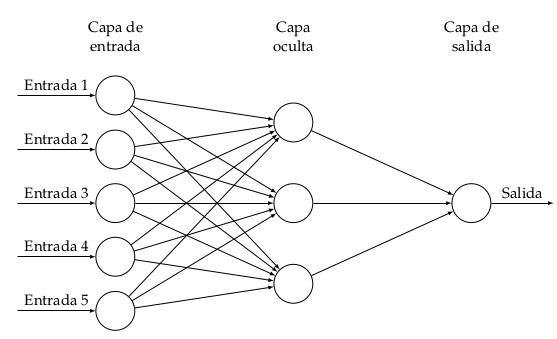
\includegraphics[width=1\textwidth]{Chapter3/neural-net}
\caption{Ejemplo de red neuronal prealimentada de cinco entradas y una salida.}
\label{fig:red-neuronal}
\end{figure}



Puesto que el objetivo del trabajo es poner en funcionamiento una modelo de clasificación multiclase no se entrará en más detalles del funcionamiento interno de este tipo de redes. No obstante, en los siguientes subapartados se explicarán algunas técnicas utilizadas durante el desarrollo del perceptrión multicapa en capítulo \ref{Chapter4}

\newpage


\subsection{Dropout}
\label{subs:dropout}

Existe una situación en la que durante el entrenamiento de un modelo podemos obtener altas tasas de acierto mientras que al usar el conjunto de validación o datos reales -es decir, cuando el software está en producción- tiene un rendimiento muy bajo, esto es debido al sobreentrenamiento (\textit{overfitting} en inglés).

Para contrarrestar este efecto se utiliza de forma extendidada técnicas como los términos de regularización L1 y L2,
que básicamente son funciones que penalizan ciertas configuraciones de parámetros \citep{xu2010l1}. No obstante,
para las redes neuronales existe otra técnica que además de ofrecer una solución al sobreentrenamiento permite
acortar los tiempos de entrenamiento. Esta técnica se denomina \textit{dropout} \citep{JMLR:v15:srivastava14a}, y consiste en, de forma aleatoria, desconectar unidades (o neuronas) de la red como se muestra en la figura \ref{fig:dropout}.

\begin{figure}[htp]
    \centering
    \begin{subfigure}[b]{0.3\textwidth}
        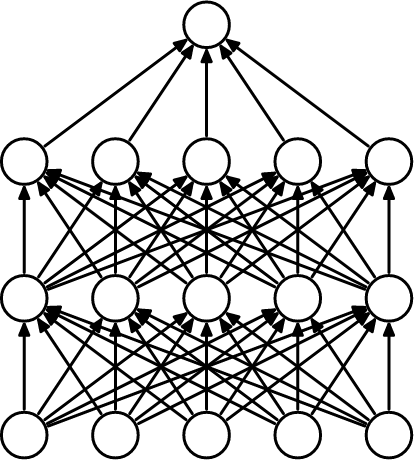
\includegraphics[width=\textwidth]{Chapter3/dropout-before}
        \caption{Red neuronal original.}
        \label{fig:dropout-before}
    \end{subfigure}
    \qquad
     %add desired spacing between images, e. g. ~, \quad, \qquad, \hfill etc.
      %(or a blank line to force the subfigure onto a new line)
    \begin{subfigure}[b]{0.3\textwidth}
        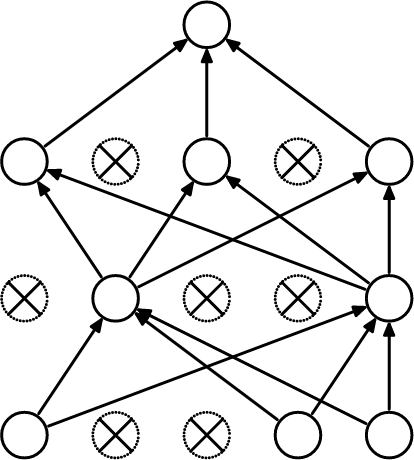
\includegraphics[width=\textwidth]{Chapter3/dropout-after}
        \caption{Despúes de aplicar \textit{dropout}.}
        \label{fig:dropout-after}
    \end{subfigure}
     %add desired spacing between images, e. g. ~, \quad, \qquad, \hfill etc.
    %(or a blank line to force the subfigure onto a new line)
    \caption{Comparación tras aplicar \textit{dropout} a una red neuronal. Las unidades marcadas con una X son las que han sido apartadas aleatoriamente en esta iteración. (Figura extraída de \citep{JMLR:v15:srivastava14a})}\label{fig:dropout}
\end{figure}



\newpage



\subsection{Inicialización Glorot}

El algoritmo Glorot (también llamado Xavier \cite{glorot2010understanding}) determina el valor de todos los pesos
iniciales de la red basándose en el número de entradas y salidas de las neuronas \cite{glorot-lasagne}. Existen distintas implementaciones para esta función, sobretodo dependiendo el programa o \textit{framework} que se utilice, aunque los autores \cite{glorot2010understanding} originalmente la definen como :

\begin{equation}
Var(W)=\frac{2}{n_{in}+n_{out}}
\end{equation}

Esta función permite regular la inicialización de los pesos de la red de forma correcta, puesto que un valor de
inicio pequeño se perdería según fuera avanzando en la red; mientras que, uno grande, iría incrementándose hasta ser
demasiado grande como para ser útil.


\subsection{Funciones no lineales}

El propósito de las funciones de activación es introducir nolinearidad a la red con tal de que las salidas no puedan ser reproducidas mediante una combinación lineal de las entradas.

A continuación se muestra alguna de las funciones utilizadas en el apartado de experimentación [\ref{sec:experimentación}] del capítulo \ref{Chapter4}.


\subsubsection{Rectificador}

Se define la función \textit{rectify} como:

\begin{equation}
f(x) = max(0, x)
\end{equation}

La figura \ref{fig:rectify} representa esta función en una gráfica para los valores de x comprendidos entre -5 y 5.

\begin{figure}[ht]
  \centering
    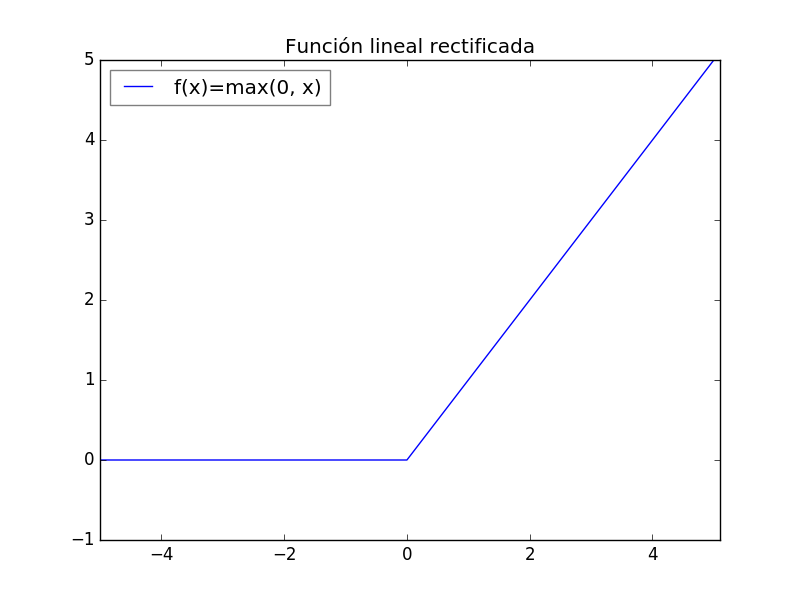
\includegraphics[width=1\textwidth]{Chapter3/rectify}
  \caption{Valores que toma la función \textit{rectify}}
\label{fig:rectify}
\end{figure}


\subsubsection{Tangente hiperbólica}

La functión \textit{tanh} se define formalmente en \ref{tanh} y su representación en un gráfico en \ref{fig:tanh}

\begin{equation}
f(x) = tanh(x)
\label{tanh}
\end{equation}

\begin{figure}[ht]
  \centering
    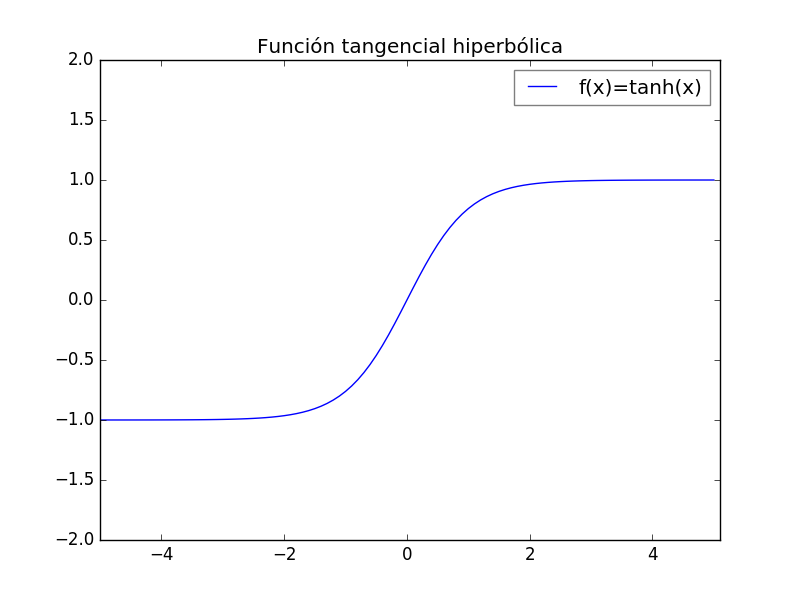
\includegraphics[width=1\textwidth]{Chapter3/tanh}
  \caption{Valores que toma la función \textit{tanh}}
\label{fig:tanh}
\end{figure}


\subsubsection{Sigmoidea}

La última función probada como función de activación en la red funcional es la función \textit{sigmoid}:

\begin{equation}
f(x)=\frac{1}{1+{e}^{-x}}
\end{equation}

Y para los valores de x entre -5 y 5, la función tiene el aspecto que se muestra en la figura \ref{fig:sigmoid}.


\begin{figure}[ht]
  \centering
    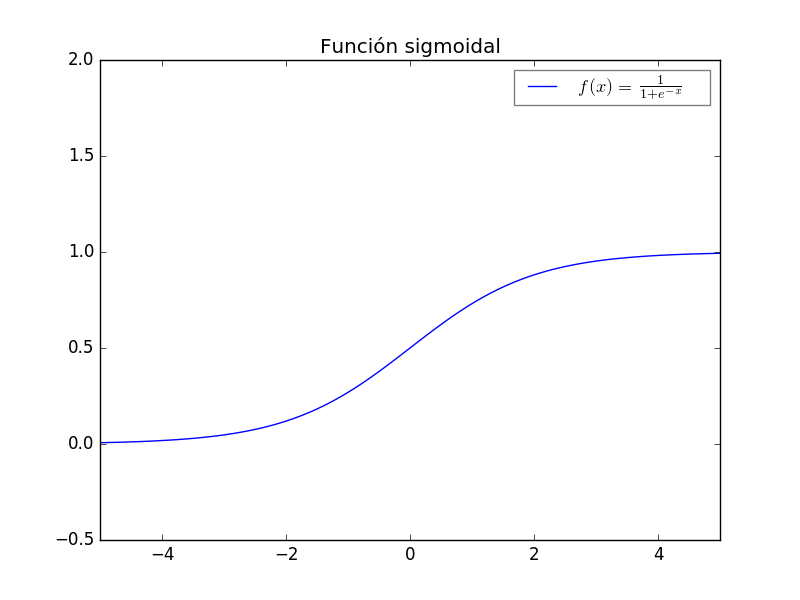
\includegraphics[width=1\textwidth]{Chapter3/sigmoid}
  \caption{Valores que toma la función \textit{sigmoid}}
\label{fig:sigmoid}
\end{figure}
